% The pass of "Render a ping without Gazebo" (render-a-ping.md), from gz_sonar/examples/render_ping.cc:
% a flat seabed with a 1 x 1 x 0.5 m box (x 9.5-10.5, y 3.5-4.5) and a 0.25 m glass float at (16, 6); two straight
% passes along +x, 3 m up, 250 pings 0.1 m apart (x 0 to 24.9).
%   sidescan (Omniscan, 50 deg tall, 20 deg down, to port, 20 m window) along y = 0: seabed from y = 3 (45 deg) to
%   y = 19.8 (range 20 m); the box shadows the seabed out to y = 4.5 * 3 / 2.5 = 5.4.
%   profiler (Surveyor, 80 deg fan across track, looking down) along y = 4, over the box: y 1.5 to 6.5.
% (a) section through the box at x = 10, looking aft, so port (+y) is to the right. True scale, 1 unit = 1 m.
% (b) plan view, +x to the right, port (+y) up.
% Build: pdflatex render_ping_pass.tex, then pdftocairo to ../images/render_ping_pass.{png,svg}
\documentclass[tikz,border=6pt]{standalone}
\usetikzlibrary{arrows.meta,calc}
\renewcommand{\familydefault}{\sfdefault}
\tikzset{
  lbl/.style={font=\sffamily\small},
  beam/.style={fill=black!7,draw=black,thin},
  dim/.style={thin,{Latex[length=1.6mm]}-{Latex[length=1.6mm]}},
  lead/.style={thin,black!70},
  axis/.style={thin,dashed},
  shadow/.style={fill=black!30,draw=none},
}
% seabed line from x0 to x1 at height z (drawing units), slab of dots below
\newcommand{\seabed}[3]{
  \draw[thick] (#1,#3) -- (#2,#3);
  \foreach \r [count=\i] in {0.12,0.3} {
    \pgfmathsetmacro{\o}{mod(\i,2)*0.12}
    \pgfmathsetmacro{\n}{int((#2-#1-0.3)/0.24)}
    \foreach \k in {0,...,\n} \fill ({#1+0.12+\k*0.24+\o},{#3-\r}) circle (0.4pt);
  }
}
% sonar head at #1, pitched down #2 degrees
\newcommand{\head}[2]{
  \begin{scope}[shift={#1},rotate=-#2]
    \draw[fill=black!15] (-0.5,-0.13) rectangle (0,0.13);
    \fill (0,0) circle (1.4pt);
  \end{scope}
}
\begin{document}
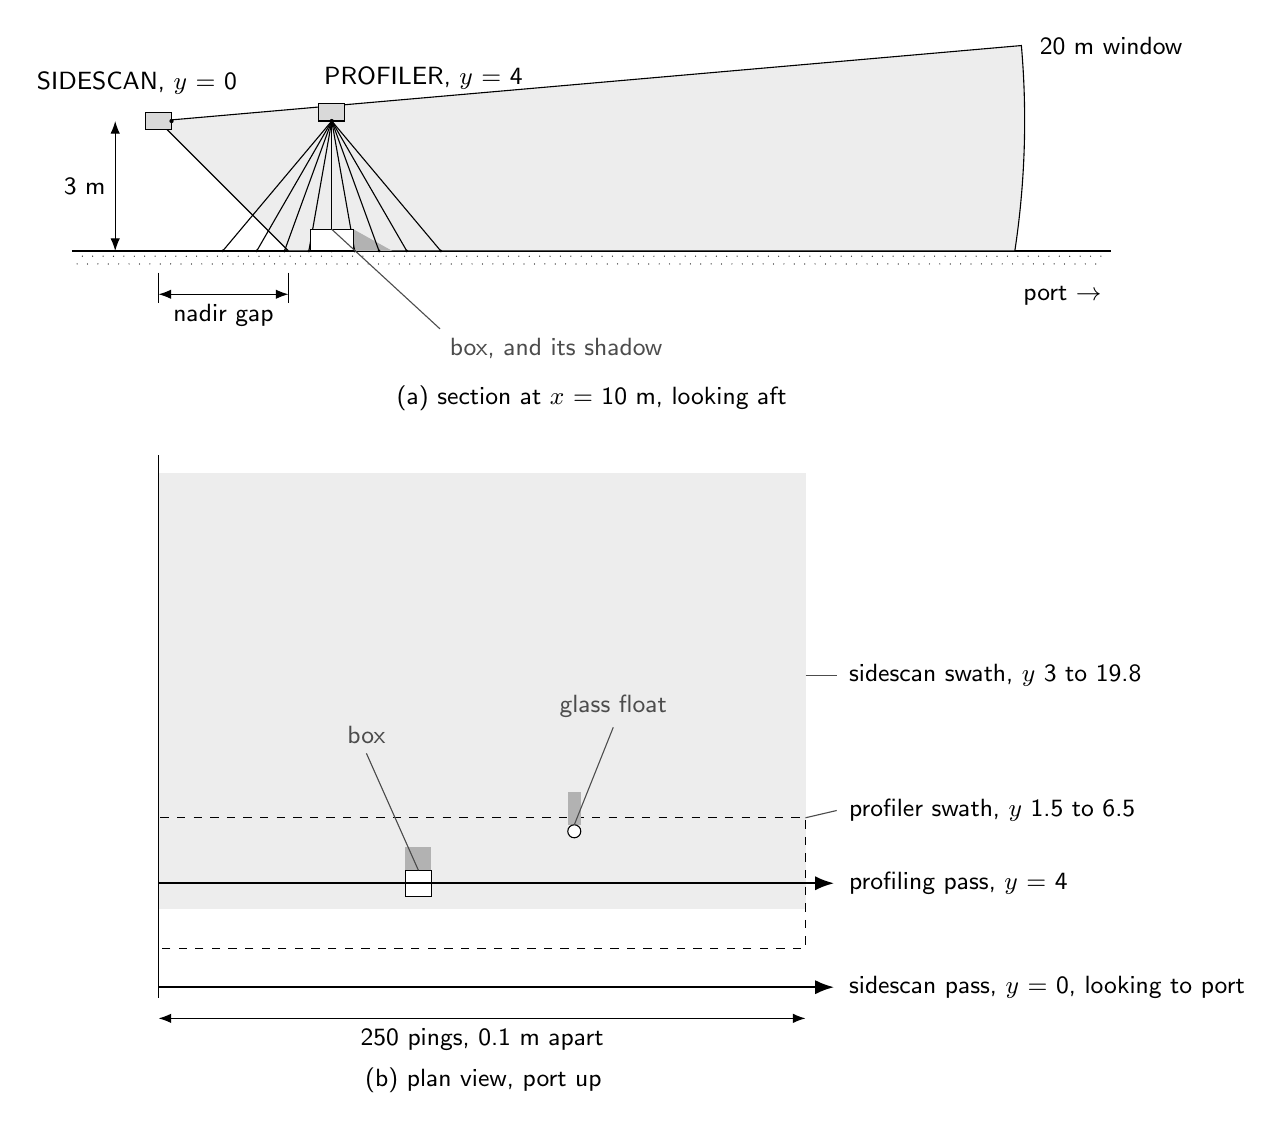
\begin{tikzpicture}[scale=0.55]
  % ---------------- (a) section at x = 10
  \begin{scope}
    \pgfmathsetmacro{\af}{asin(3/20)}
    \seabed{-2}{22}{0}
    \draw[beam] (0,3) -- ({20*cos(5)},{3+20*sin(5)}) arc (5:-\af:20) -- (3,0) -- cycle;
    \fill[shadow] (4.5,0.5) -- (5.4,0) -- (4.5,0) -- cycle;
    \foreach \t in {-40,-30,...,40} {
      \draw[thin] (4,3) -- ({4+3*tan(\t)},0);
      \fill ({4+3*tan(\t)},0) circle (1pt);
    }
    \draw[fill=white] (3.5,0) rectangle (4.5,0.5);
    \draw[fill=black!15] (-0.3,2.8) rectangle (0.3,3.2); \fill (0.3,3) circle (1.4pt);
    \draw[fill=black!15] (3.7,3) rectangle (4.3,3.4); \fill (4,3) circle (1.4pt);
    \draw[dim] (-1,3) -- (-1,0) node[lbl,midway,left] {3 m};
    \draw[dim] (0,-1) -- (3,-1) node[lbl,midway,below] {nadir gap};
    \draw (0,-0.5) -- (0,-1.2) (3,-0.5) -- (3,-1.2);
    \node[lbl,anchor=west] at ({20*cos(5)+0.2},{3+20*sin(5)}) {20 m window};
    \node[lbl,anchor=south] at (-0.5,3.4) {SIDESCAN, $y$ = 0};
    \node[lbl,anchor=south west] at (3.6,3.5) {PROFILER, $y$ = 4};
    \draw[lead] (4,0.5) -- (6.5,-1.8) node[lbl,anchor=north west] {box, and its shadow};
    \node[lbl,anchor=north east] at (22,-0.6) {port $\rightarrow$};
    \node[lbl] at (10,-3.4) {(a) section at $x$ = 10 m, looking aft};
  \end{scope}
  % ---------------- (b) plan view
  \begin{scope}[shift={(0,-17)},scale=0.6]
    \fill[black!7] (0,3) rectangle (24.9,19.77);
    \draw[dashed] (0,1.48) rectangle (24.9,6.52);
    \fill[shadow] (9.5,4.5) rectangle (10.5,5.4);
    \fill[shadow] (15.75,6.25) rectangle (16.25,7.5);
    \draw[fill=white] (9.5,3.5) rectangle (10.5,4.5);
    \draw[fill=white] (16,6) circle (0.25);
    \draw[thick,-{Latex[length=2.4mm]}] (0,0) -- (26,0);
    \draw[thick,-{Latex[length=2.4mm]}] (0,4) -- (26,4);
    \draw (0,-0.4) -- (0,20.5);
    \node[lbl,anchor=west] at (26.2,0) {sidescan pass, $y$ = 0, looking to port};
    \node[lbl,anchor=west] at (26.2,4) {profiling pass, $y$ = 4};
    \node[lbl,anchor=west] at (26.2,12) {sidescan swath, $y$ 3 to 19.8};
    \draw[lead] (24.9,12) -- (26.1,12);
    \node[lbl,anchor=west] at (26.2,6.8) {profiler swath, $y$ 1.5 to 6.5};
    \draw[lead] (24.9,6.52) -- (26.1,6.8);
    \draw[lead] (10,4.5) -- (8,9) node[lbl,anchor=south] {box};
    \draw[lead] (16,6.25) -- (17.5,10) node[lbl,anchor=south] {glass float};
    \draw[dim] (0,-1.2) -- (24.9,-1.2) node[lbl,midway,below] {250 pings, 0.1 m apart};
    \node[lbl] at (12.5,-3.6) {(b) plan view, port up};
  \end{scope}
\end{tikzpicture}
\end{document}
